Based on the implementation of the SOME/IP technology, the applications are run on the target hardware to realize the outcome. In this chapter, the results of several scenarios of the technology are presented and a brief overview of the troubleshooting guide is discussed.

\subsection{Server Application Output}
The server application is running on the virtual machine, and Figure \ref{fig:res_server_eth0} shows the server application's log information. The virtual machine is linked to the network via an Ethernet cable to a router that serves as a gateway.

\begin{figure}[!htb]
	\centering
		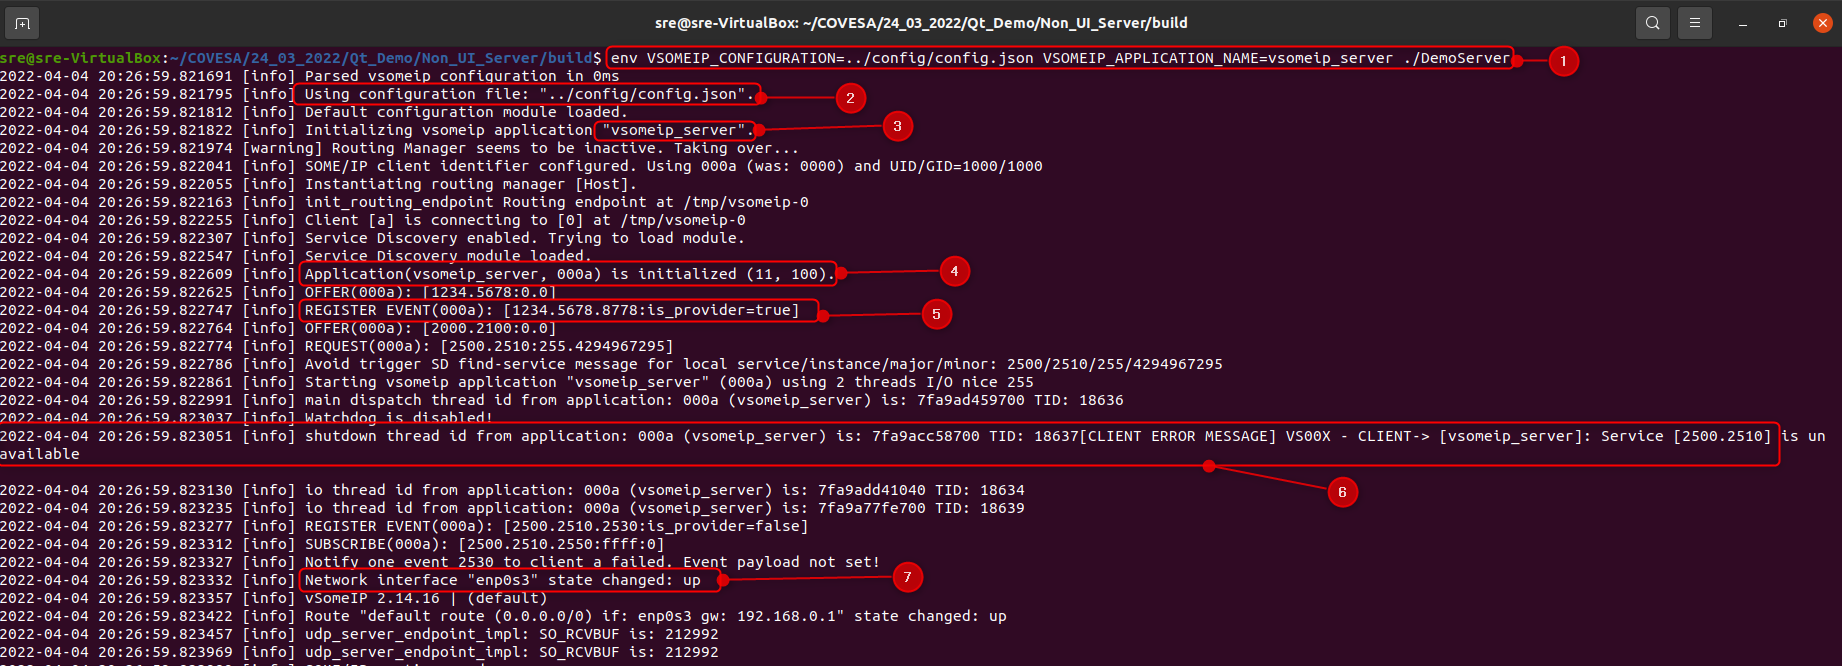
\includegraphics[width=1\textwidth, height=6cm, keepaspectratio]{images/res_server_eth0.png}
	\caption{Inter-ECU SOME/IP communication demonstration - Server}
	\label{fig:res_server_eth0}
\end{figure}

In the figure \ref{fig:res_server_eth0}, several important information fields are denoted by numbers. The number 1 represents the initial configuration of the environment, which includes the configuration file name, the application name, and the executable name. These are required to launch the vsomeip application in order to establish inter-ECU communication. Number 2 indicates that the configuration file was found and the load was successful after the application was successfully executed. After that, the application is initialized, and the services are provided if the initialization is successful. When the variable \textquote{is field} is set to true, it indicates that the event being offered is a field-based event. To provide an event that is not field-based, the variable must be set to false. The marking numbers 3, 4, and 5 in the figure \ref{fig:res_server_eth0} all point to these specifics. Number 6 indicates that when a service request was made, the service with ID 0x2500 and instance ID 0x2510 was unavailable. This error can occur if the vsomeip application that provides this service is unavailable and the service details are not found in the service registry. When all of the applications are not launched at the same time, such occurrences are fairly common. These types of errors and symptoms are covered in the troubleshooting guide and will be covered in the subsequent sections. Marking number 7 indicates that the Ethernet connection was successfully established and that the target hardware can now communicate with other target hardware running vsomeip applications on the same network.

\subsection{Client Application Output},
The client application, like the server application, must be executed. The environment configurations, on the other hand, are not required if multiple applications are to be run on the same machine. Figure \ref{fig:res_client_1_eth0} shows an example of log data from a client application to demonstrate an application running on the same device (intra-ECU communication). The most important information is highlighted in the image and explained in this section.

\begin{figure}[!htb]
	\centering
		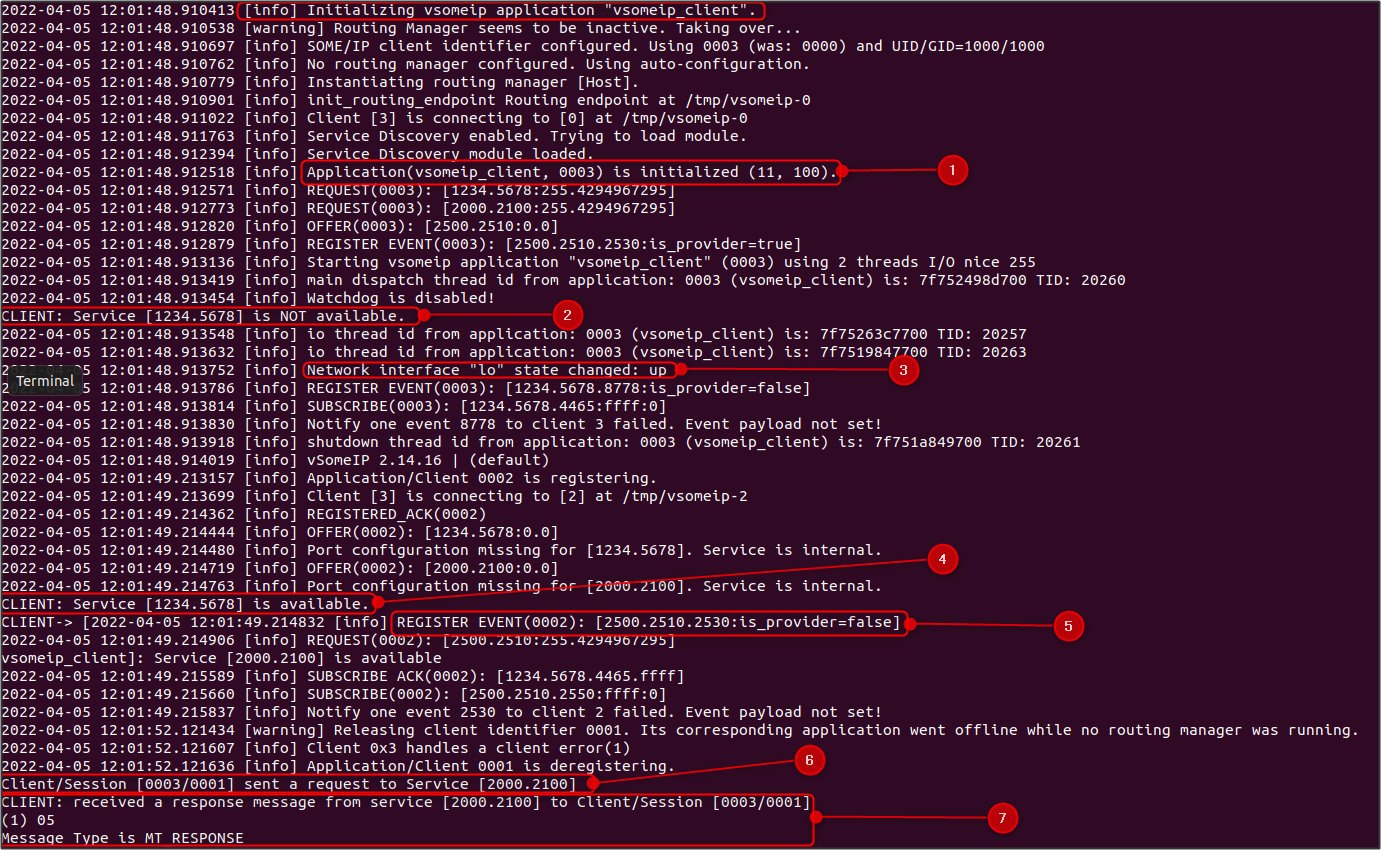
\includegraphics[width=1\textwidth, height=7cm, keepaspectratio]{images/res_client_1_eth0.png}
	\caption{Example of Inter-ECU SOME/IP communication - Client}
	\label{fig:res_client_1_eth0}
\end{figure}

\par The number 1 indicates that an application with the name \textquote{vsomeip\_client} has been started. Following initialization, a request to service 0x1234 is sent. The server details, on the other hand, were not found in the registry, and the same information is denoted by the marking number 2. The third marking indicates that the client application is running on the same device, namely the local host. If the application is running on another device, log information similar to that of the server application output should be displayed. When the application providing service 0x1234 is active, the client application detects the service's availability and adds it to the local service registry.The service is then ready for use, and additional data requests can be made to it. Marking number 4 displays information about service availability. The number 5 indicates that the client application is offering an event with ID 0x2530 from service 0x2500 and that the event is registered in the database. Furthermore, data requests can be made once the relevant services are available and registered. The number 6 in the diagram indicates that a message request to service 0x2000 with service instance 0x2100 was sent. The server then responds by sending a message containing the requested data, depending on the type of message request. The communication method used in the case denoted by marking number 7 is request-response, and the response message received is of the type “MT\_RESPONSE”. Similarly, event notifications are sent based on the frequency specified in the application or a change in the data.

\subsection{Troubleshooting guide}
Although user guide documentation for newer technologies is available, it is a challenge to set up and implement the technology. When it came to setting up the system and successfully running the applications on the target hardware during the development of the SOME/IP technology, there were many challenges. Some of these challenges were related to library and stack installation, which are well covered in the vsomeip stack user guide\cite{b_vsomeip_userguide}. However, several errors were discovered during the application's development and testing phases. Some of these errors can be caused by an incorrect method of implementing software code, while others can be caused by an improper configuration of the stack and applications. To avoid such issues in the future while developing SOME/IP-based applications, commonly encountered issues have been documented in the form of a troubleshooting guide. Each error message in this troubleshooting guide is assigned an error code, as well as the possible root cause and method for resolving the problem. Figure \ref{fig:troubleshooting_guide} depicts a section of the troubleshooting guide. The error messages displayed while running the applications are investigated, and the possible root cause and solutions are documented. This guide can be used by other developers who are using SOME/IP stacks provided by different vendors to try to replicate the issues using the demonstrator in order to better understand the problems.

\begin{figure}[!htb]
	\centering
		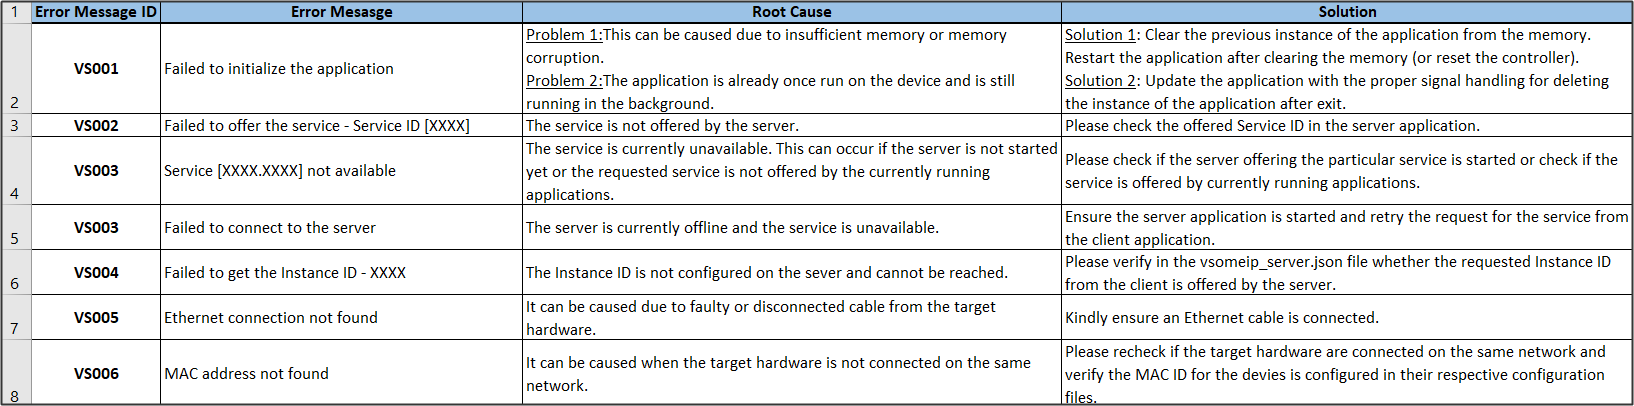
\includegraphics[width=1\textwidth]{images/troubleshooting_guide.png}
	\caption{SOME/IP troubleshooting guide}
	\label{fig:troubleshooting_guide}
\end{figure}
